\documentclass[conference]{IEEEtran}
\IEEEoverridecommandlockouts
% The preceding line is only needed to identify funding in the first footnote. If that is unneeded, please comment it out.
\usepackage{cite}
\usepackage{amsmath,amssymb,amsfonts}
\usepackage{algorithmic}
\usepackage{graphicx}
\usepackage{textcomp}
\usepackage{xcolor}
\def\BibTeX{{\rm B\kern-.05em{\sc i\kern-.025em b}\kern-.08em
    T\kern-.1667em\lower.7ex\hbox{E}\kern-.125emX}}
\begin{document}

\title{Conference Paper Title*\\
{\footnotesize \textsuperscript{*}Note: Sub-titles are not captured in Xplore and
should not be used}
\thanks{Identify applicable funding agency here. If none, delete this.}
}

% \author{\IEEEauthorblockN{1\textsuperscript{st} Given Name Surname}
% \IEEEauthorblockA{\textit{dept. name of organization (of Aff.)} \\
% \textit{name of organization (of Aff.)}\\
% City, Country \\
% email address or ORCID}
% \and
% \IEEEauthorblockN{2\textsuperscript{nd} Given Name Surname}
% \IEEEauthorblockA{\textit{dept. name of organization (of Aff.)} \\
% \textit{name of organization (of Aff.)}\\
% City, Country \\
% email address or ORCID}
% \and
% \IEEEauthorblockN{3\textsuperscript{rd} Given Name Surname}
% \IEEEauthorblockA{\textit{dept. name of organization (of Aff.)} \\
% \textit{name of organization (of Aff.)}\\
% City, Country \\
% email address or ORCID}
% \and
% \IEEEauthorblockN{4\textsuperscript{th} Given Name Surname}
% \IEEEauthorblockA{\textit{dept. name of organization (of Aff.)} \\
% \textit{name of organization (of Aff.)}\\
% City, Country \\
% email address or ORCID}
% \and
% \IEEEauthorblockN{5\textsuperscript{th} Given Name Surname}
% \IEEEauthorblockA{\textit{dept. name of organization (of Aff.)} \\
% \textit{name of organization (of Aff.)}\\
% City, Country \\
% email address or ORCID}
% \and
% \IEEEauthorblockN{6\textsuperscript{th} Given Name Surname}
% \IEEEauthorblockA{\textit{dept. name of organization (of Aff.)} \\
% \textit{name of organization (of Aff.)}\\
% City, Country \\
% email address or ORCID}
% }

\maketitle

% \begin{abstract}
% This document is a model and instructions for \LaTeX.
% This and the IEEEtran.cls file define the components of your paper [title, text, heads, etc.]. *CRITICAL: Do Not Use Symbols, Special Characters, Footnotes, 
% or Math in Paper Title or Abstract.
% \end{abstract}

% \begin{IEEEkeywords}
% component, formatting, style, styling, insert
% \end{IEEEkeywords}

\section{Introduction}
This document is a model and instructions for \LaTeX.
Please observe the conference page limits. 

\section{Literature review}

\subsection{U-Net}
\subsubsection{Introduction of U-Net}
Ronneberger, Fischer and Brox [1] developed a convolutional network named U-Net, which comprise a contracting path and a symmetric expanding path enabling this network to capture context and precise localization. Moreover, U-Net require few images to train end-to-end and the calculating speed for this architecture is very fast. It can segment a 512x512 image within a second on a up to data GPU.

\subsubsection{U-Net architecture and mechanism}
\centerline{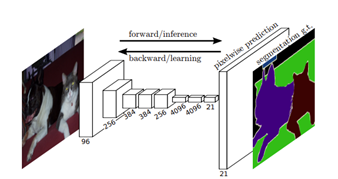
\includegraphics[width=40mm,scale=0.5]{group/Picture1.png}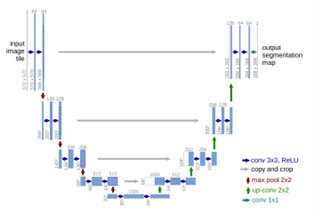
\includegraphics[width=40mm,scale=0.5]{group/Picture2.png}}
\textbf{Network Architecture}: The network architecture is illustrated in Figure 1 (b). The whole network formed by two parts, the contracting path (left side) and expansive path (right side). A typical convolutional network is followed by the contracting path. The contracting path includes a repeated implementation of two 3x3 convolutions (unpadded convolutions), each accompanied by a rectified linear unit (ReLU) and a 2x2 max pooling operation downsampling for 2 strides. For each downsampling step, this architecture replicates the number of feature channels. Each step in the expansive path comprises upsampling the feature map, followed by a 2x2 convolution (“up-convolution”) that splits the number of feature channels into two parts. This is then linked with the correspondingly cropped feature map from the contracting path followed by two 3x3 convolutions, each accompanied by a ReLU activation. The last final layer is a 1x1 convolution mapping each 64-component feature vector to the number of requested categories. There are 23 convolution layers in this structure.
\textbf{Mechanism}: The U-Net architecture consisting of a contracting path and an expansive path developed from the so-called “fully convolutional network” [2] (see Figure 1 a). Boosting a usual contracting network by successive layers is the basic concept in fully convolutional network [2], which the upsampling operators substitute the pooling operators. Therefore, these successive layers enhance the output resolution. In order to achieve the function of localization, the upsampled output ally with the high-resolution features generated from the contracting path. A more accurate output based on the information above can be assembled by the successive convolution layer.
One significant modification in the U-Net architecture is that the upsampling part contains a huge quantities of feature channels, empowering the higher resolution layers to capture context information. As a result, the expansive path is approximately symmetric to the contracting path, structuring a u-shaped network. Besides, the U-Net architecture only uses the valid part of each convolution, which means that it does not contain any fully connected layers. The scheme provides an overlap-tile strategy for seamless segmentation of any large images

\subsection{DeeplabV3}
Semantic segmentation, aimed at assigning semantic labels to every pixel in an image, is one of the fundamental topics in computer vision [14]. The encoder-decoder network has been successfully applied to numerous computer vision tasks, including object detection [12] and semantic segmentation [11]. Typically, the encoder-decoder network consists of two components: an encoder module that gradually reduces the feature maps and captures higher-level semantic information, and a decoder module that gradually recovers spatial information. The autoencoder model fully adheres to this concept [15], while U-Net incorporates skip connections between the encoder and decoder to effectively obtain sharper segmentations.

\subsubsection{Depthwise Separable Convolution}
Depthwise separable convolution or group convolution serves as a powerful operation to reduce both computation costs and the number of parameters while maintaining comparable performance [19]. This operation has been adopted in many recent neural network designs, such as flattened convolutional neural networks and the Xception model[17], showing improvements in both accuracy and speed for the task of semantic segmentation.

\subsubsection{Deep Convolutional Neural Networks and the DeepLab Series}
Deep convolutional neural networks based on Fully Convolutional Networks (FCNs) demonstrate significant improvements over systems relying on hand-crafted features in benchmark tasks [18]. DeepLabv3 utilizes several parallel atrous convolutions with different rates, known as Atrous Spatial Pyramid Pooling (ASPP)[19]. However, due to the design of state-of-the-art neural networks and limited GPU memory, it becomes computationally prohibitive to extract output feature maps that are 8 or 4 times smaller than the input resolution. The DeepLabv3+ model extends DeepLabv3 by adding an effective decoder module to recover object boundaries, allowing for detailed recovery of object contours [11].
\subsubsection{Long-Range Context Modeling}
One approach to enhancing the ability of convolutional neural networks (CNNs) to model long-range dependencies is through the adoption of self-attention [21] or non-local modules [20]. However, these methods notoriously consume vast memory resources to compute the large affinity matrix at each spatial position. Other strategies for long-range context modeling include dilated convolutions [22], which aim to widen the receptive field of CNNs without introducing additional parameters. A common limitation of these methods, including dilated convolutions and pooling, is that they probe input feature maps within square windows. Qinbin proposed a strip pooling module that narrows the pooling window [25], allowing the model to collect rich global contextual information and increase the receptive field of the backbone network; he also presented a mixed pooling module based on the classic residual block with a bottleneck structure.
\subsubsection{Residual Networks and Their Variants}
Furthermore, Targ et al. proposed a novel residual architecture known as ResNet-in-ResNet (RiR)[24], which incorporates residual blocks within the framework of a ResNet. The advantage of this model is the optimization benefits stemming from skip connections; however, the implementation requires tuning of additional parameters. Recent studies have also supported the notion that deep residual networks function akin to ensembles of relatively shallow networks [26], revealing the existence of exponential paths from the output layer to the input layer that gradient information can follow. Masoud introduced multi-residual networks that increase the multiplicity of the network while keeping its depth fixed[23].
Therefore, employing DeepLabv3+ for image segmentation can provide numerous advantages in terms of performance and cost-effectiveness. Strip pooling is lightweight and can serve as an efficient plug-and-play module for existing segmentation models. Multi-residual networks enhance the number of residual functions within the residual blocks, resulting in networks that are wider rather than deeper, thereby facilitating parallelism to reduce the computational cost of the network. Hence, we propose an improved DeepLabv3+ model that integrates strip pooling and multi-residual layers, which can offer numerous benefits in terms of efficiency and robustness, making it a promising option for a wide range of applications.
\subsection{Mask R-CNN}
Mask R-CNN first passes a feature map generated to the Region Proposal Network (RPN), applies a sliding window across the feature map, and uses pre-defined anchor boxes to potential object bounding boxes that possibly contain objects. In contrast to RoIPool, which reduces proposed regions to a consistent size via quantisation in Fast R-CNN, mask R-CNN introduces RoIAlign, a pixel-to-pixel alignment mechanism as mask predictions require more accurate and precise spatial features. Extracted features will be passed through a pre-trained convolutional neural network. For each region of interest, a set of bounding boxes and class labels are predicted independent of pixel-wise masks as mask prediction will occur in parallel in the new branch of Mask R-CNN. Mask R-CNN is an extension of Fast R-CNN, originally used for object detection and will only generate bounding boxes and identify object classes. The key improvements from Fast R-CNN to Mask R-CNN are applying a mask branch for instance segmentation, introducing RoI Align to preserve pixel accuracy and adopting a multi-task loss function that combines loss of classification, segmentation and position. These improvements allow Mask R-CNN to perform well in instance segmentation tasks and lay out the foundation of application on our dataset.
\section{Method}
To evaluate models with “SeaTurtleID2022” dataset, we train, validate, and test models using three different architecture and mechanism (attention and residual learning). We compare the performance of ResUNet++, DeeplabV3, and Mask RCNN.
for you.
\subsection{U-Net with Attention Gate and Deep Residual Learning}
\subsubsection{Attention (machine learning)}
Attention is a machine learning method for attending to an input vector’s different parts to catch long-term dependencies. According to the background of 
\centerline{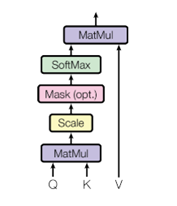
\includegraphics[width=40mm,scale=0.5]{group/Picture3.png}}
Figure 2. Scaled Dot-Product Attention
Natural Language Processing (NLP), standard sequence-to-sequence models squeezed the input sequence to a fixed-length context vector, which obstructed their capability to remember long inputs, for example, sentences. On the other hand, attention produces shortcuts between the context vector and the entire source input [3]
\subsubsection{Attention Gate}
Attention Gate (AG) [5] is a variant of Attention mechanism concentrates on targeted regions while repressing feature activations in unrelated regions.
Figure 3. Schematic of the proposed additive Attention Gate [5].
\centerline{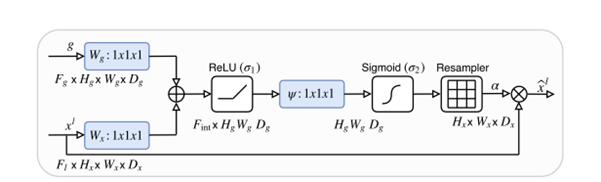
\includegraphics[width=40mm,scale=0.5]{group/Picture4.png}}
Given the input feature map X and the gating signal $G∈R^(C^'×H×W)$ which is collected at a broad scale and holds contains contextual information, the attention gate utilizes additive attention to acquire the gating coefficient. Both the gating signal and the input X are initially mapped linearly to an $R^(F×H×W)$ dimensional space, after that, a spatial attention weight map $S∈R^(1×H×W)$ is generated by compressing the output in the channel domain.
The overall process can be written as:
$$
\begin{aligned}
    S&=σ(φ(δ(ϕ_x (X)+ϕ_g (G))))\\
    Y&=SX
\end{aligned}
$$
Where $φ$, $ϕ_x$ and $ϕ_g$ are linear transformations implemented as 1 × 1 convolution
\subsubsection{Residual Learning}
Residual Neural Network, also known as Residual Network or ResNet, is a deep learning architecture that the weight layers learn residual functions with reference to the layer inputs. One of the most important terminologies named “residual connection” refers to the specific architectural motif of $x↦f(x)+x$, in which f is an arbitrary neural network module [4].
\subsubsection{Deep Residual U-Net}
Deep Residual U-Net, also called as Deep ResUNet. It is a semantic segmentation neural network build with residual units and has similar architecture of U-Net [6].
\centerline{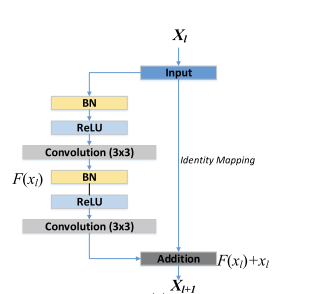
\includegraphics[width=40mm,scale=0.5]{group/Picture5.png}}
Figure 4. Residual unit with identity mapping used in the ResUnet [6].
The residual neural network includes a number of stacked residual units. The residual unit can be described as a form:
$$
\begin{aligned}
    y_l&=h(x_l)+F(x_l,w_l)\\
    x_(l+1)&=f(y_l)
\end{aligned}
$$
Where $x_l$ and $x_(l+1)$ are the input and output of the lth residual unit. F, f and h are the residual function, activation function and identity mapping function respectively.
Through the residual unit, Zhengxin et al.(2018) [6] built a deep ResUnet architecture as shown in Fig. 5. This network structure combines two benefits 
Figure 5. Architecture of deep ResUnet[6].
\centerline{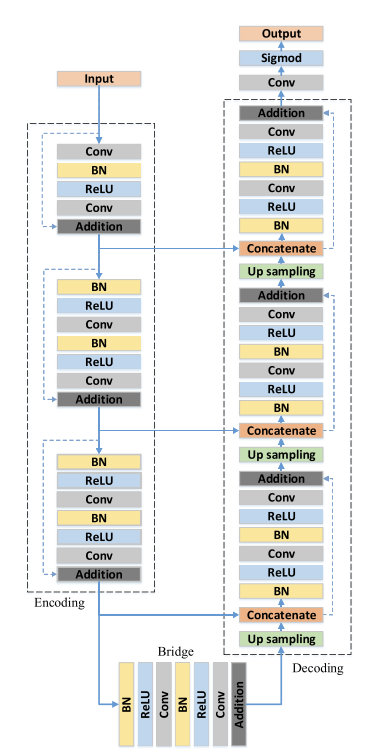
\includegraphics[width=40mm,scale=0.5]{group/Picture6.png}}
From different aspects. First, the residual unit allows an ease training of this network. Second, the residual unit combined with the skip connections between low levels and high levels of the network will assist information propagation without degradation. Which brings us a possibility to develop a neural network with a significant fewer parameters.
\subsubsection{ResUNet++}
\centerline{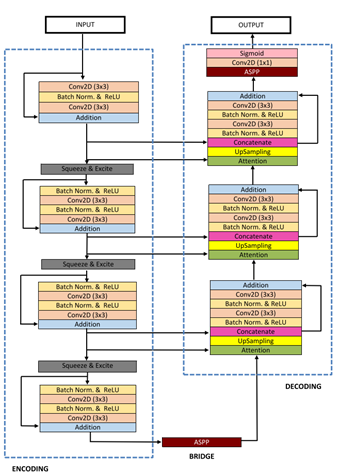
\includegraphics[width=40mm,scale=0.5]{group/Picture7.png}}
Based on the information above, Debesh et al. (2019) [7] raised a segmentation architecture that utilizes the advantage of deep residual learning and attention gate with U-Net.
Figure 6. Architecture of ResUNet++[7].
\subsection{DeeplabV3+}
\subsubsection{Segmentation Network}
Previous studies have demonstrated that DeepLabV3+ can achieve remarkable segmentation results [11]. Therefore, it is optimized in this study as the benchmark model for turtle segmentation. The block diagram of the DeeplabV3 plus segmentation model is illustrated in Figure 8. The model comprises two main components: an encoder and a decoder.
To effectively extract features of turtles from the given images, the encoder includes a backbone network and an improved Atrous Spatial Pyramid Pooling (ASPP). The backbone network utilizes ResNet101. We propose an improved ASPP performs parallel operations of improved multi-residual atrous convolution with varying dilation rates and enhanced strip pooling, instead of regular atrous convolution and global average pooling. Specifically, three 3x3 convolutions are performed with dilation rates of 6, 12, and 18, respectively. These variations expand the receptive field and improve localization detection accuracy without losing resolution. This operation condenses the features extracted by the improved backbone network into multi-scale contextual semantic information. 
In the decoder, the output features of the encoder are first bilinearly upsampled by a factor of 4, followed by a concatenation with the low-level features from the improved backbone in the channel dimension. To reduce the number of channels in the low-level features, a 1x1 convolution is applied prior to concatenation, followed by a 3x3 convolution operation to refine the features. Finally, a bilinear upsampling operation by a factor of 4 is performed to yield the final semantic segmentation results.
\centerline{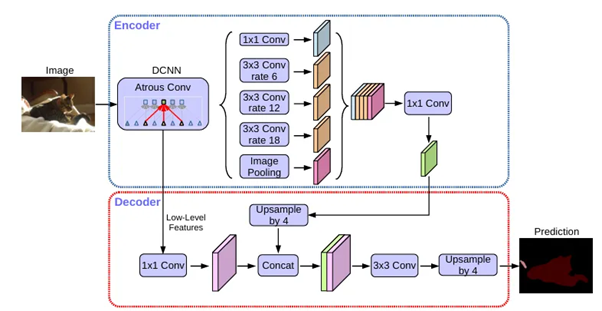
\includegraphics[width=80mm,scale=0.5]{group/Picture8.png}}
\subsubsection{Improved multi-residual atrous convolution}
The improved multi-residual atrous convolution integrates two multiscale residual blocks while introducing dilation to preserve the features of atrous convolution [23]. This approach provides several benefits, including enhanced feature extraction, minimized overfitting, superior resolution adaptability, a wider network structure, and improved handling of class imbalances. By utilizing two parallel multiscale dilated residual blocks with varying scale parameters, dual multiscale residual blocks can capture a broader range of features across different input image scales, resulting in diverse and complementary feature learning. The parallel arrangement of dual multiscale residual blocks also promotes gradient flow during backpropagation as illustrated in Figure 8, thereby aiding in training deeper networks and alleviating the vanishing gradient issue. Overall, dual multiscale residual with dilatated ratio blocks present a robust and efficient methodology for image segmentation tasks by leveraging multiple scales, expanding the receptive field and refined feature extraction. 
\centerline{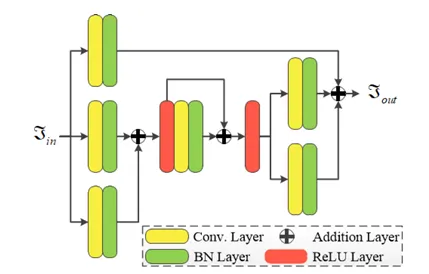
\includegraphics[width=40mm,scale=0.5]{group/Picture9.png}}
\subsubsection{Strip Pooling Module}
The Strip Pooling Module leverages both horizontal and vertical strip pooling operations to capture long-range context from various spatial dimensions [15]. Initially, the input tensor x is fed into two parallel pathways, each containing either a horizontal or vertical strip pooling layer followed by a 1D convolutional layer with a kernel size of 3, which modulates the current location and its neighboring features.
During this process, each position in the output tensor can establish relationships with a variety of positions in the input tensor. For example, as illustrated in Figure 9, the square bounded by the black box in the output tensor is connected to all locations that share the same horizontal or vertical coordinates (enclosed by the red and purple boxes). Therefore, by repeating the above aggregation process multiple times, it becomes possible to build long-range dependencies across the entire scene. Moreover, benefiting from the element-wise multiplication operation, the proposed Strip Pooling Module can also be considered an attention mechanism and can be directly applied to any pretrained backbone networks without the need to retrain them from scratch [15].
\centerline{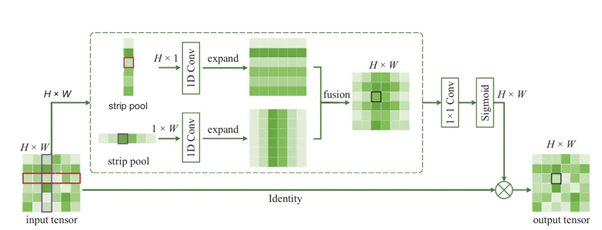
\includegraphics[width=80mm]{group/Picture10.png}}
\subsection{Mask R-CNN}
Mask R-CNN was chosen due to its effectiveness in mask prediction and its novel application of instance segmentation techniques to semantic segmentation tasks. Mask R-CNN achieves state-of-the-art performance in instance segmentation, making it a strong candidate for tasks requiring accurate mask localization. While models like U-Net and DeepLabv3 are often used directly for semantic segmentation, applying Mask R-CNN leverages its robust instance segmentation capabilities creatively. The use of a multi-task loss function also enhances mask prediction accuracy by allowing better localization. 
The Mask R-CNN model uses ResNet50 with a Feature Pyramid (FPN) as its backbone, initialized with pre-trained weights. The FastRCNNPredictor and MaskRCNNPredictor heads are modified to adapt four output classes: background, carapace, flipper, and head. Experimental dropout is applied after the linear layers in the box prediction head to prevent overfitting, as the model tends to converge quickly.
\subsection{Preparing the Dataset}
In this study, we utilize the image dataset from SeaTurtleID2022, which contains a total of 438 individual sea turtles. To enhance the robustness and enrich our dataset, we employed several augmentation strategies, including random rotation, random cropping, random brightness and contrast adjustments, random blurring, and noise addition, among others. Image preprocessing was performed to reduce computational costs and improve efficiency. All images were uniformly resized to 512 x 512 pixels. The dataset used in this research was divided into training, validation, and testing subsets according to an open-set splitting file. This open-set splitting provides a significant increase on realistic performance evaluation compared to random splitting or closed-set splitting [8]. 
\subsection{Loss Function}
In this study, we observed that the head and legs have a significantly smaller number of pixels compared to the background. The carapace, while larger than the head and legs, is still smaller than the background. The frequency differences among the four categories can cause an imbalance during training, which may lead to the underestimation of the importance of target pixels. Therefore, a combined loss function was employed in this study, consisting of class-weighted Dice loss, class-weighted focal loss, and class-weighted cross-entropy loss. The final weights assigned to the dataset are 0.02 for the head, 0.21 for the legs, 0.63 for the carapace, and 1.0 for the background.
Class-weighted Dice loss is particularly effective in addressing imbalances in class distribution. It measures the overlap between the predicted and ground truth segmentations, emphasizing the importance of smaller classes by weighting them differently. This is beneficial in cases where certain classes (like the head and legs) are underrepresented.
Class-weighted focal loss is designed to address the issue of class imbalance by focusing more on hard-to-classify examples. It consists of a modulating factor that reduces the relative loss for well-classified examples, putting more focus on challenging cases. This property is especially useful in tasks involving high variability in class frequencies, helping the model better learn from those difficult instances.
Class-weighted cross-entropy loss is a widely used loss function in classification tasks. By applying class weights, it allows the model to give more importance to less frequent classes while still ensuring a standard probabilistic interpretation of the predicted classifications. This can help achieve a balanced learning process across all classes.
The weights are calculated using the following formula:
$$
W_m=N(\frac{mean fre}{fre_m })
$$
where $fre_m$ represents the frequency of occurrences of pixels in class mm divided by the total number of pixels in any image containing that class and mean $fre$  denotes the mean of these frequencies across each image. N is the normalization factor for all weights. Therefore, the overall loss function is formulated as:
$$
loss=p*dice+q*focal+z*cross
$$
where dice is the Dice loss, focal is the focal loss, and cross is the cross-entropy loss. The constants p,q,z are used to balance the contributions of the three loss components.

\subsection{Implementation Details}
All architectures were implemented using the TensorFlow frame [9]. We performed our experiment on a single GPU RTX A6000 (NVIDIA). The training system is part of Additive Manufacturing Laboratories heterogeneous cluster and has an Intel(R) 13th Gen Core (TM) i9-13900K CPU 3.00 GHz, 128G of DDR4-2667MHz DRAM. We start the training with a batch size of 8, and the proposed architectures are optimized by Adam optimizer. We set a learning rate adjustment schedule with 1e-4 as the beginning rate. This schedule will increase the learning rate to 1e-3 empowering models to have a better learning outcome. After this model reached the max learning rate, the schedule will decrease it on the later part of the training to prevent overfitting.
\newpage
\subsection{Abbreviations and Acronyms}\label{AA}
Define abbreviations and acronyms the first time they are used in the text, 
even after they have been defined in the abstract. Abbreviations such as 
IEEE, SI, MKS, CGS, ac, dc, and rms do not have to be defined. Do not use 
abbreviations in the title or heads unless they are unavoidable.

\subsection{Units}
\begin{itemize}
\item Use either SI (MKS) or CGS as primary units. (SI units are encouraged.) English units may be used as secondary units (in parentheses). An exception would be the use of English units as identifiers in trade, such as ``3.5-inch disk drive''.
\item Avoid combining SI and CGS units, such as current in amperes and magnetic field in oersteds. This often leads to confusion because equations do not balance dimensionally. If you must use mixed units, clearly state the units for each quantity that you use in an equation.
\item Do not mix complete spellings and abbreviations of units: ``Wb/m\textsuperscript{2}'' or ``webers per square meter'', not ``webers/m\textsuperscript{2}''. Spell out units when they appear in text: ``. . . a few henries'', not ``. . . a few H''.
\item Use a zero before decimal points: ``0.25'', not ``.25''. Use ``cm\textsuperscript{3}'', not ``cc''.)
\end{itemize}

\subsection{Equations}
Number equations consecutively. To make your 
equations more compact, you may use the solidus (~/~), the exp function, or 
appropriate exponents. Italicize Roman symbols for quantities and variables, 
but not Greek symbols. Use a long dash rather than a hyphen for a minus 
sign. Punctuate equations with commas or periods when they are part of a 
sentence, as in:
\begin{equation}
a+b=\gamma\label{eq}
\end{equation}

Be sure that the 
symbols in your equation have been defined before or immediately following 
the equation. Use ``\eqref{eq}'', not ``Eq.~\eqref{eq}'' or ``equation \eqref{eq}'', except at 
the beginning of a sentence: ``Equation \eqref{eq} is . . .''

\subsection{\LaTeX-Specific Advice}

Please use ``soft'' (e.g., \verb|\eqref{Eq}|) cross references instead
of ``hard'' references (e.g., \verb|(1)|). That will make it possible
to combine sections, add equations, or change the order of figures or
citations without having to go through the file line by line.

Please don't use the \verb|{eqnarray}| equation environment. Use
\verb|{align}| or \verb|{IEEEeqnarray}| instead. The \verb|{eqnarray}|
environment leaves unsightly spaces around relation symbols.

Please note that the \verb|{subequations}| environment in {\LaTeX}
will increment the main equation counter even when there are no
equation numbers displayed. If you forget that, you might write an
article in which the equation numbers skip from (17) to (20), causing
the copy editors to wonder if you've discovered a new method of
counting.

{\BibTeX} does not work by magic. It doesn't get the bibliographic
data from thin air but from .bib files. If you use {\BibTeX} to produce a
bibliography you must send the .bib files. 

{\LaTeX} can't read your mind. If you assign the same label to a
subsubsection and a table, you might find that Table I has been cross
referenced as Table IV-B3. 

{\LaTeX} does not have precognitive abilities. If you put a
\verb|\label| command before the command that updates the counter it's
supposed to be using, the label will pick up the last counter to be
cross referenced instead. In particular, a \verb|\label| command
should not go before the caption of a figure or a table.

Do not use \verb|\nonumber| inside the \verb|{array}| environment. It
will not stop equation numbers inside \verb|{array}| (there won't be
any anyway) and it might stop a wanted equation number in the
surrounding equation.

\subsection{Some Common Mistakes}\label{SCM}
\begin{itemize}
\item The word ``data'' is plural, not singular.
\item The subscript for the permeability of vacuum $\mu_{0}$, and other common scientific constants, is zero with subscript formatting, not a lowercase letter ``o''.
\item In American English, commas, semicolons, periods, question and exclamation marks are located within quotation marks only when a complete thought or name is cited, such as a title or full quotation. When quotation marks are used, instead of a bold or italic typeface, to highlight a word or phrase, punctuation should appear outside of the quotation marks. A parenthetical phrase or statement at the end of a sentence is punctuated outside of the closing parenthesis (like this). (A parenthetical sentence is punctuated within the parentheses.)
\item A graph within a graph is an ``inset'', not an ``insert''. The word alternatively is preferred to the word ``alternately'' (unless you really mean something that alternates).
\item Do not use the word ``essentially'' to mean ``approximately'' or ``effectively''.
\item In your paper title, if the words ``that uses'' can accurately replace the word ``using'', capitalize the ``u''; if not, keep using lower-cased.
\item Be aware of the different meanings of the homophones ``affect'' and ``effect'', ``complement'' and ``compliment'', ``discreet'' and ``discrete'', ``principal'' and ``principle''.
\item Do not confuse ``imply'' and ``infer''.
\item The prefix ``non'' is not a word; it should be joined to the word it modifies, usually without a hyphen.
\item There is no period after the ``et'' in the Latin abbreviation ``et al.''.
\item The abbreviation ``i.e.'' means ``that is'', and the abbreviation ``e.g.'' means ``for example''.
\end{itemize}
An excellent style manual for science writers is \cite{b7}.

\subsection{Authors and Affiliations}
\textbf{The class file is designed for, but not limited to, six authors.} A 
minimum of one author is required for all conference articles. Author names 
should be listed starting from left to right and then moving down to the 
next line. This is the author sequence that will be used in future citations 
and by indexing services. Names should not be listed in columns nor group by 
affiliation. Please keep your affiliations as succinct as possible (for 
example, do not differentiate among departments of the same organization).

\subsection{Identify the Headings}
Headings, or heads, are organizational devices that guide the reader through 
your paper. There are two types: component heads and text heads.

Component heads identify the different components of your paper and are not 
topically subordinate to each other. Examples include Acknowledgments and 
References and, for these, the correct style to use is ``Heading 5''. Use 
``figure caption'' for your Figure captions, and ``table head'' for your 
table title. Run-in heads, such as ``Abstract'', will require you to apply a 
style (in this case, italic) in addition to the style provided by the drop 
down menu to differentiate the head from the text.

Text heads organize the topics on a relational, hierarchical basis. For 
example, the paper title is the primary text head because all subsequent 
material relates and elaborates on this one topic. If there are two or more 
sub-topics, the next level head (uppercase Roman numerals) should be used 
and, conversely, if there are not at least two sub-topics, then no subheads 
should be introduced.

\subsection{Figures and Tables}
\paragraph{Positioning Figures and Tables} Place figures and tables at the top and 
bottom of columns. Avoid placing them in the middle of columns. Large 
figures and tables may span across both columns. Figure captions should be 
below the figures; table heads should appear above the tables. Insert 
figures and tables after they are cited in the text. Use the abbreviation 
``Fig.~\ref{fig}'', even at the beginning of a sentence.

\begin{table}[htbp]
\caption{Table Type Styles}
\begin{center}
\begin{tabular}{|c|c|c|c|}
\hline
\textbf{Table}&\multicolumn{3}{|c|}{\textbf{Table Column Head}} \\
\cline{2-4} 
\textbf{Head} & \textbf{\textit{Table column subhead}}& \textbf{\textit{Subhead}}& \textbf{\textit{Subhead}} \\
\hline
copy& More table copy$^{\mathrm{a}}$& &  \\
\hline
\multicolumn{4}{l}{$^{\mathrm{a}}$Sample of a Table footnote.}
\end{tabular}
\label{tab1}
\end{center}
\end{table}

\begin{figure}[htbp]
\centerline{\includegraphics{fig1.png}}
\caption{Example of a figure caption.}
\label{fig}
\end{figure}

Figure Labels: Use 8 point Times New Roman for Figure labels. Use words 
rather than symbols or abbreviations when writing Figure axis labels to 
avoid confusing the reader. As an example, write the quantity 
``Magnetization'', or ``Magnetization, M'', not just ``M''. If including 
units in the label, present them within parentheses. Do not label axes only 
with units. In the example, write ``Magnetization (A/m)'' or ``Magnetization 
\{A[m(1)]\}'', not just ``A/m''. Do not label axes with a ratio of 
quantities and units. For example, write ``Temperature (K)'', not 
``Temperature/K''.

\section*{Acknowledgment}

The preferred spelling of the word ``acknowledgment'' in America is without 
an ``e'' after the ``g''. Avoid the stilted expression ``one of us (R. B. 
G.) thanks $\ldots$''. Instead, try ``R. B. G. thanks$\ldots$''. Put sponsor 
acknowledgments in the unnumbered footnote on the first page.

\section*{References}

Please number citations consecutively within brackets \cite{b1}. The 
sentence punctuation follows the bracket \cite{b2}. Refer simply to the reference 
number, as in \cite{b3}---do not use ``Ref. \cite{b3}'' or ``reference \cite{b3}'' except at 
the beginning of a sentence: ``Reference \cite{b3} was the first $\ldots$''

Number footnotes separately in superscripts. Place the actual footnote at 
the bottom of the column in which it was cited. Do not put footnotes in the 
abstract or reference list. Use letters for table footnotes.

Unless there are six authors or more give all authors' names; do not use 
``et al.''. Papers that have not been published, even if they have been 
submitted for publication, should be cited as ``unpublished'' \cite{b4}. Papers 
that have been accepted for publication should be cited as ``in press'' \cite{b5}. 
Capitalize only the first word in a paper title, except for proper nouns and 
element symbols.

For papers published in translation journals, please give the English 
citation first, followed by the original foreign-language citation \cite{b6}.

\begin{thebibliography}{00}
\bibitem{b1} G. Eason, B. Noble, and I. N. Sneddon, ``On certain integrals of Lipschitz-Hankel type involving products of Bessel functions,'' Phil. Trans. Roy. Soc. London, vol. A247, pp. 529--551, April 1955.
\bibitem{b2} J. Clerk Maxwell, A Treatise on Electricity and Magnetism, 3rd ed., vol. 2. Oxford: Clarendon, 1892, pp.68--73.
\bibitem{b3} I. S. Jacobs and C. P. Bean, ``Fine particles, thin films and exchange anisotropy,'' in Magnetism, vol. III, G. T. Rado and H. Suhl, Eds. New York: Academic, 1963, pp. 271--350.
\bibitem{b4} K. Elissa, ``Title of paper if known,'' unpublished.
\bibitem{b5} R. Nicole, ``Title of paper with only first word capitalized,'' J. Name Stand. Abbrev., in press.
\bibitem{b6} Y. Yorozu, M. Hirano, K. Oka, and Y. Tagawa, ``Electron spectroscopy studies on magneto-optical media and plastic substrate interface,'' IEEE Transl. J. Magn. Japan, vol. 2, pp. 740--741, August 1987 [Digests 9th Annual Conf. Magnetics Japan, p. 301, 1982].
\bibitem{b7} M. Young, The Technical Writer's Handbook. Mill Valley, CA: University Science, 1989.
\end{thebibliography}
\vspace{12pt}
\color{red}
IEEE conference templates contain guidance text for composing and formatting conference papers. Please ensure that all template text is removed from your conference paper prior to submission to the conference. Failure to remove the template text from your paper may result in your paper not being published.

\end{document}
